\section*{Введение}
\addcontentsline{toc}{section}{\protect Введение}%
IN PROGRESS...


\section{Описание конструкции реактора}
IN PROGRESS...



\section{Теплофизический расчет}

\subsection{Постановка задачи}
В данном разделе будут определены основные термодинамические и гидравлические параметры реакторной установки. Теплофизический расчет подразумевает следующий ряд задач:

    \begin{enumerate}
        \item Выбор турбины и разработка принципиальной теплосиловой схемы установки;
        \item Рассчет КПД проектируемой установки;
        \item Рассчет основных теплофизических характеристик, таких как мощность ТВС и твэла, расход и скорсоть теплоносителя, коэффициент теплоотдачи;
        \item Построение распределения температур теплоносителя, оболочки и топлива по длинне для наиболее напряжённого канала; 
        \item Определение максимально возможных температур теплоносителя, оболочки и топлива;
        \item Рассчёт энергозатраты на собственные нужды и уточнение КПД;
        \item Рассчёт коэффициента запаса до кризиса теплообмена;
    \end{enumerate}

\subsection{Исходные данные для проведения расчетов}


Для проведения теплогидравлического расчета реакторной установки использовались следующие характеристики, представленные в Таблице \ref{tabular:data}.

\begin{table}[H]
	\caption{Исходные данные для проектируемого РУ ВВЭР-1000}
	\begin{center}
        \begin{tabular}{|l|c|}
        \toprule
         Характеристика & Значение \\ 
         \midrule
         \hline
         Электрическая мощность реактора, МВт & 1000 \\
         \hline\ 
         Температура теплоносителя на входе в АЗ,$^\circ C$  & 287 \\ 
         \hline\
         Температура теплоносителя на выходе АЗ, $^\circ C$ & 320 \\ 
         \hline
         Температура питательной воды, , $^\circ C$ & 220 \\ 
         \hline
         Температура свежего пара, $^\circ C$  &  281 \\ 
         \hline
         Давление свежего пара & 6.5 \\ 
         \hline
         Температура пара после пароперегревателей, $^○C$ & 250 \\ 
         \hline
         Давление в АЗ, МПа & 15.7 \\ 
         \hline
         Степень сухости пара прсле ЦВД и ЦНД, \% & 80 \\ 
         \hline
         Количество петель РУ & 4 \\ 
         \hline
         Число ТВС, шт & 163 \\ 
         \hline
         Число твэл в ТВС, шт & 317 \\ 
         \hline
         Коэффициент неравномерности по высоте АЗ & 1.5 \\ 
         \hline
         Коэффициент неравномерности по радиусу АЗ & 1.25 \\ 
         \hline
         Высота АЗ, м & 3.5 \\ 
         \hline
         Диаметр твэл, мм & 9.1 \\ 
         \hline
         Размер ТВС «под ключ», мм & 234 \\ 
         \hline
         Диаметр центрального канала в ТВС, мм & 10.3 \\ 
         \hline
         Число направляющих каналов в ТВС, шт & 12 \\ 
         \hline
         Шаг решетки ТВС, мм & 12,75 \\ 
         \hline
         Диаметр направляющего канала в ТВС, мм & 12.6 \\ 
         \hline
         Толщина оболочки твэл, мм & 0.65 \\ 
         \hline
         Толщина газового зазора в твэл, мм & 0.135 \\ 
         \hline
         Диаметр топливной таблетки, мм. & 7.53 \\ 
         \hline
         Диаметр отверстия топливной таблетки, мм & 1.3 \\ 
         \bottomrule
		\end{tabular}
		\label{tabular:data}
	\end{center}
\end{table}




\subsection{Выбор турбины}
В качестве турбины в расчетах будем использовать модель К-1000-60/1500-2. Её характеристики представлены в таблице \ref{tabular:turbine}


\begin{table}[H]
	\caption{Параметры турбины К-1000-60/1500-2 }
	\begin{center}
        \begin{tabular}{|l|c|}
        \toprule
         Параметр & Значение или Название \\ 
         \midrule
         \hline
         Прототип турбины &  К-1000-60/1500\\ 
         \hline
         Температура питательной воды, $^\circ C$ & 220 \\ 
         \hline
         Температура свежего пара, $^\circ C$  & 281\\ 
         \hline
         Давление свежего пара, $^\circ C$ & 6.5 \\ 
         \hline
         Температура после промежуточного перегрева, $^○C$ & 250 \\ 
         \hline
         Количество регенеративных подогревателей & 7 \\ 
         \bottomrule
		\end{tabular}
		\label{tabular:turbine}
	\end{center}
\end{table}


\begin{figure}[H]
	\begin{center}
		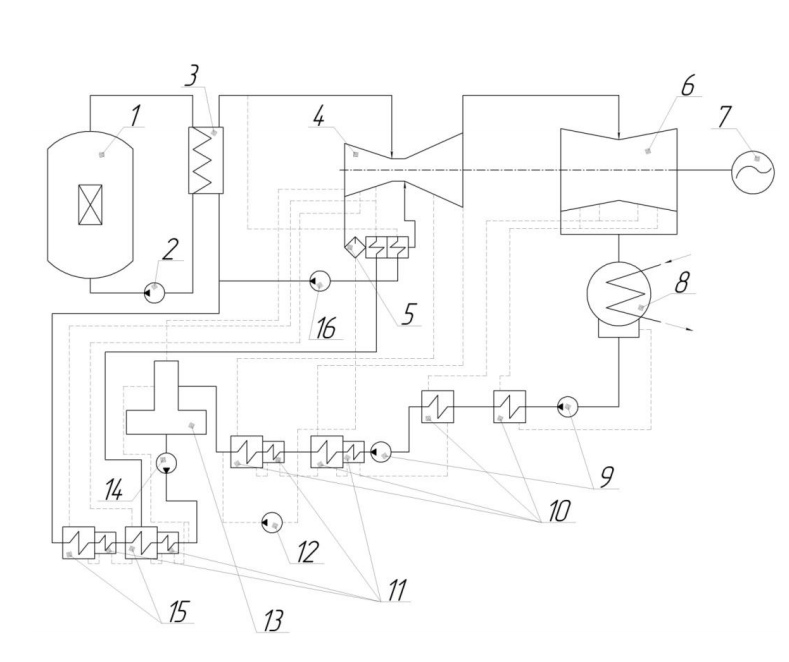
\includegraphics[scale=0.5]{teploscheme.jpg}
		\caption{Тепловая схема АЭС: 1 – ядерный реактор, 2 – главный
циркуляционный насос, 3 – парогенератор, 4 – цилиндр высокого давления, 5 –
сепаратор-пароперегреватель, 6 – цилиндры низкого давления, 7 – генератор, 8
– конденсатор, 9 – конденсационный электронасос, 10 – подогреватель низкого
давления, 11 – охладитель, 12 – станция насосная, 13 – деаэратор, 14 –
плунжерный электронасос, 15 – подогреватель высокого давления, 16 –
конденсационный насос с гидротурбинным приводом}
		\label{pic:teplocheme} % название для ссылок внутри кода
	\end{center}
\end{figure}


\subsection{Расчет КПД термодинамического цикла}


\begin{figure}[H]
	\begin{center}
		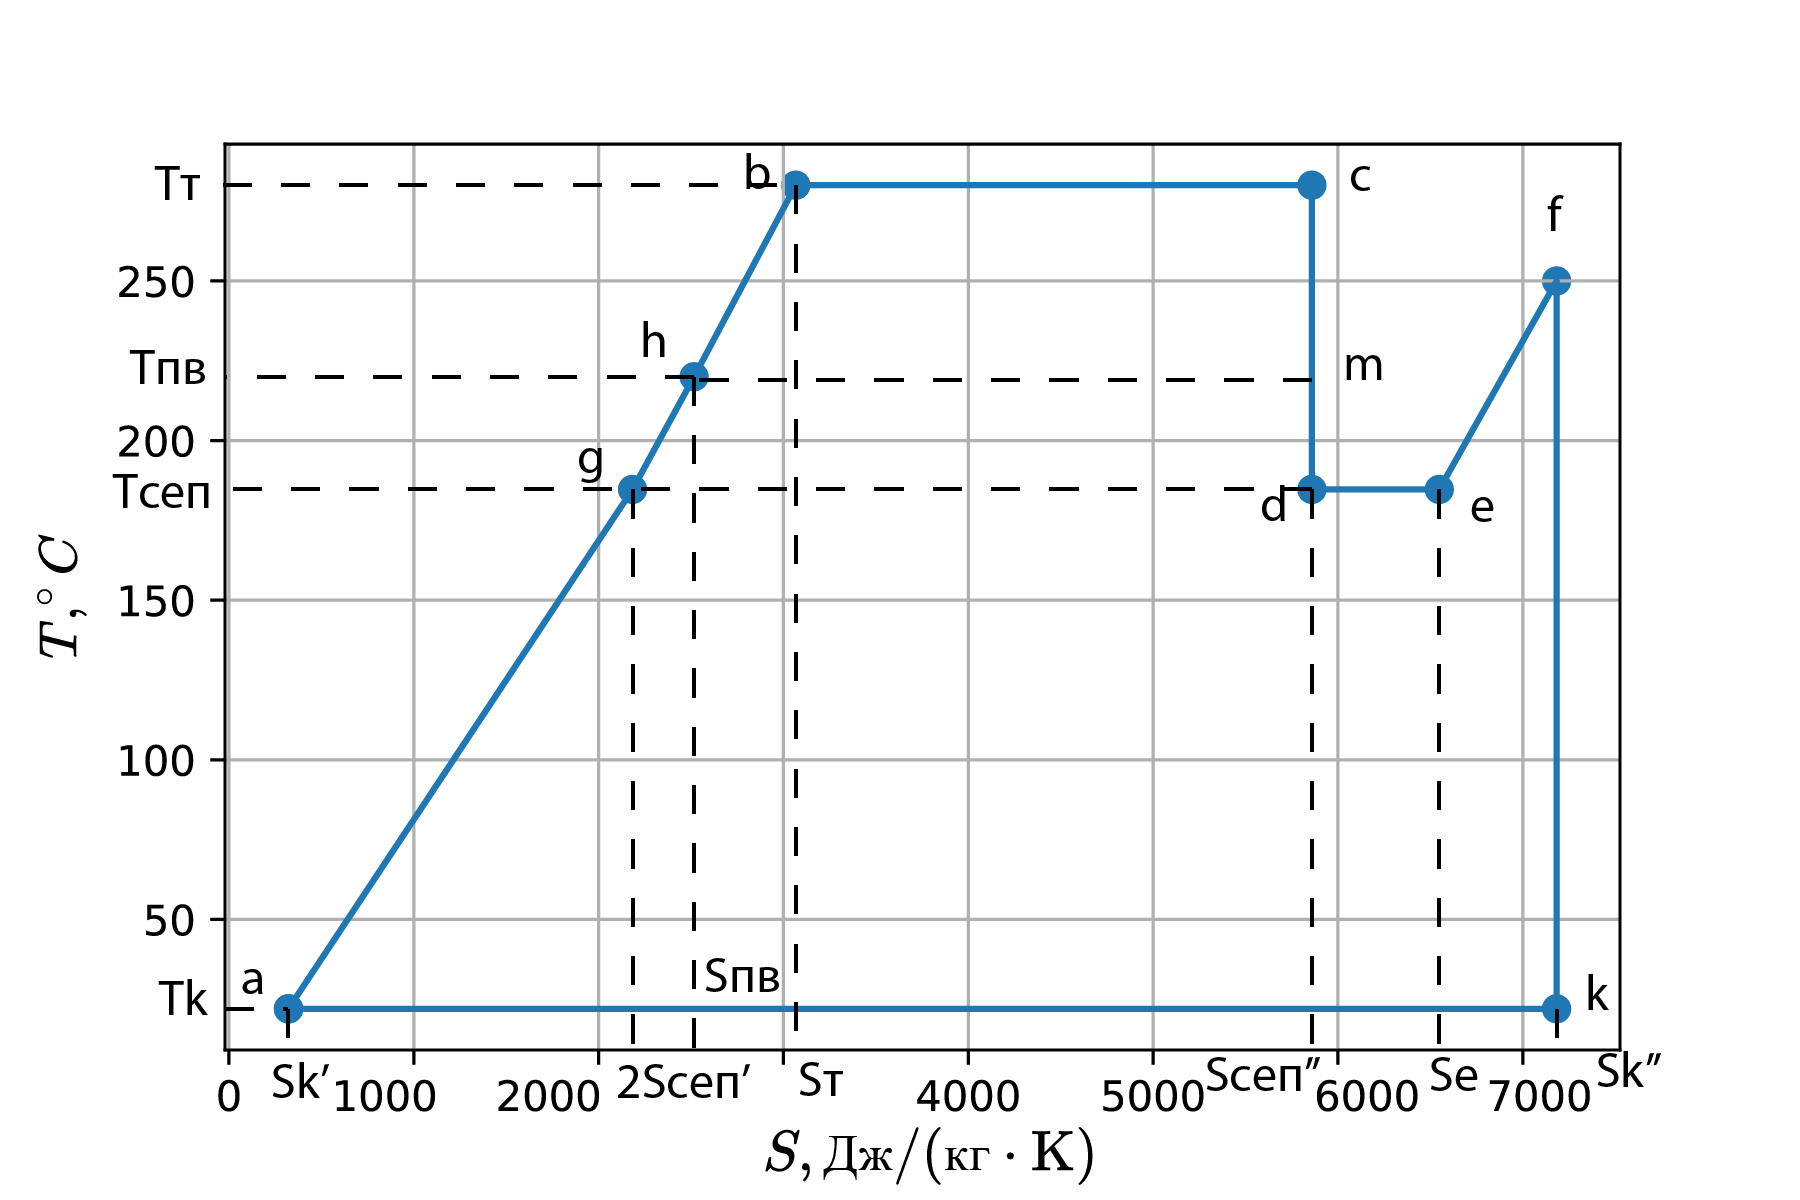
\includegraphics[scale=0.15]{TS.png}
		\caption{ T­S диаграмма турбинного цикла в реакторе ВВЭР­1000 : hbc —нагрев и испарение в парогенераторе; cd — расширение пара в ЦВД; de — паротделяется от конденсата в сепараторе; ef — пар поступает в промежуточныйпароперегреватель; fk — расширение пара в ЦНД; ka ­ конденсация в конден­саторе; ag — регенеративный подогрев в ПНД; gh — регенеративный подогревв ПВД6
        }
		\label{pic:TS} % название для ссылок внутри кода
	\end{center}
\end{figure}

\begin{table}[H]
	\caption{Значения параметров TS-диаграммы}
	\begin{center}
        \begin{tabular}{|c|c|c|c|c|}
        \toprule
         Точка & P, МПа & T, $^\circ C$ & S, Дж/(кг*К) & h, кДж/кг \\ 
         \midrule
         \hline
          h &  2.6 & 220 & 2517 & 943.7\\ 
         \hline
          b & 6.5 & 281 & 3076 & 2780 \\ 
         \hline
          c & 6.5 & 281 & 5852 & 2779\\ 
         \hline
          d & 1.13 & 185 & 5852 & 2465 \\ 
         \hline
          e & 1.13 & 185 & 6543 & 2782 \\ 
         \hline
          f & 1.13 & 250  & 6863 & 2938 \\ 
         \hline
          k & 0.0023 & 20 & 6863 & 1998 \\ 
         \hline
          k′ & 0.0023 & 20 & 295.2 & 83.92 \\ 
         \hline
          a & 6.5 & 20 & 295.2 & 90 \\ 
         \hline
          g & 1.13 & 185 & 2188 & 785.3 \\ 
         \bottomrule
		\end{tabular}
		\label{tabular:coeffs}
	\end{center}
\end{table}

Произведём расчет КПД для турбины К-1000-60/1500. Термический КПД без регенерации:
$$
η_{t0} = 1 -
\frac{T_{k} ⋅ \left( s_{f} - s_{a} \right) ⋅ x_{d}}
{\left( h_{c} - h_{g} \right) +x_{d}\left( \left( h_{g} - h_{a} \right) + \left( h_{f} - h_{e} \right) \right)} = 0.424
%= \VAR{KPD_t0}
$$
Термический КПД с идеальной регенерацией:
$$
η_{t∞} = 1 -
\frac{T_{k} ⋅ \left( s_{f} - s_{g} \right) \left( s_{c} - s_{h} \right)}
{\left(h_{c} - h_{h}\right) ⋅ \left( s_{e} - s_{g} \right) + \left( h_{f} - h_{e} \right) ⋅ \left( s_{f} - s_{h} \right)} = 0.473
%= \VAR{KPD_t∞}
$$
Термический КПД с $n = 7$  регенеративными отборами:
$$
η_{tn} = η_{t0} + \left( η_{t∞} - η_{t0} \right) ⋅ \frac{n}{n+1} = 0.467
%= \VAR{KPD_tn}
$$

Учитываем:
$\eta^{\text{вн}}$ = 0.85 — внутренний КПД турбины;
$\eta_{\text{ос}}$ = 0.98 — коэффициент использования тепла, учитывающий; потери тепла в окружающую среду в прочем энергооборудовании;
$\eta_{\text{эг}}$ = 0.98 — КПД электрогенератора;
$\eta_{\text{мех}}$ = 0.97 — КПД механический,
Вычисляем КПД брутто АЭС как:
$$
\eta_{\text{брутто}} = \eta^7 \cdot \eta^{\text{вн}} \cdot \eta_{\text{ос}} \cdot \eta_{\text{эг}} \cdot \eta_{\text{мех}} = 0.37
$$
Тепловая мощность реактора при номинальной электрической мощности $Q_{\text{эл}} = 1000$ МВт равна:
$$
Q_{\text{теп}} = \frac {Q_{\text{эл}}} {\eta^{\text{брутто}}} = 2700 МВт 
$$


\subsection{Расчет изменения теплового потока в наиболее нагруженном канале}
Из условия $K_z = \frac 1 {\int_{-H_{\text{аз}}/2}^{H_{\text{аз}}/2} \cos \left( \frac {\pi \cdot z} {H_{\text{эф}}}\right)dz} = 1.5$ находим эфективную добавку к высоте активной зоны. Эффективная высота активной зоны будет равна $H_{\text{эф}} = 2.66$ м. Максимальная величина теплового потока на один твэл:
$$
q_{max} = \frac {Q_{\text{теп}}K_r K_z}{N_{ТВС}N_{\text{твэл}}H_{\text{аз}}} = 279.93\  \frac {\text{Вт}} {\text{см}}
$$ 
Зависимость величины теплового потока от высоты:
$$
q(z) = q_{max}\cos\left(\frac {\pi\cdot z} {H_{\text{эф}}}\right) = 279.93 \cos \left(\frac {\pi \cdot z} {266} \right)\ \left[\frac{\text{Вт}}{\text{см}} \right]
$$

\subsection{Расчет распределения температуры теплоносителя по высоте}

Энтальпия входа $h_{\text{вх}} =1.268 \cdot 10^6 \frac{Дж}{кг}$.%из wsp через F(P,T) температуру на входе и давление в АЗ.

\noindent Энтальпия выхода $h_{\text{вых}} =1.453 \cdot 10^6 \frac{Дж}{кг}$. %аналогично 

\noindent Расход теплоносителя через ТВС:
$$
G_{ТВС} = \frac {Q_{\text{теп}}} {(h_{\text{вх}} - h_{\text{вх}})N_{\text{ТВС}}} = [[B43]] 
$$

\subsection{Расчет температуры топлива}

\subsection{Расчет мощности, необходимой на прокачку теплоносителя}

% \subsection{Определение запаса до кризиса теплообмена}

\subsection{Выводы из теплофизического расчета}


% \section{Нейтронно-физический расчет}
